\chapter{Анализ методов измерения и компенсации реактивного момента}\label{ch:ch1}
\section{Состояние исследований в области динамических воздействий на оптико-электронные системы КА}

В последние годы в научной инженерной среде возрастает интерес к повышению точности и разрешающей способности космических средств наблюдения, предназначенных для дистанционного зондирования Земли (ДЗЗ) и определения малоэнергетических целей \cite{haroon2020multisized, bouwmeester2023enabling, saunders2017building, cheng2024geometric, hamm2015earth}. Одним из основных направлений является увеличение размеров оптических систем и внедрения механизмов изменения положения визирной оси без поворота КА \cite{kandepi2024agile, franze2023attitude}. Подобные решения реализованы в системах типа SPOT, Pleiades-1A/1B, KOMPSAT-2. В пользовательской документации указываются допустимые значения \blur{я}, обычно в пределах $0,1-0,2$ пикселя матрицы фотоприёмника \cite{SPOT2013, Pleiades2012,KOMPSAT2008} 

Поворот визирной оси может выполняться различными способами:
\begin{itemize}
	\item разворотом всего КА;
	\item перемещением отдельных элементов оптической системы;
	\item использованием карданных механизмов \cite{leskov2010kardan,negro2023inertial}
\end{itemize}

Независимо от выбранной схемы, перемещение подвижных масс вызывает возникновение реактивных сил и моментов, передающихся на корпус аппарата, вызывая угловые отклонения и колебания. Это затрудняет работу системы стабилизации, а также снижает пространственное разрешение и контрастность изображения за счет \blur{я} и вибрационных искажений  \cite{lappas2002attitude, углова2019оценка, zhao2023effect} Особенно критично это для инфракрасных и широкоформатных систем, имеющих большие габариты и массу \cite{shorthill1990infrared, shivanandan1985far,pittelkau2012pointing, dennehy2021spacecraft, alvarez2018spacecraft}.

Таким образом, динамические возмущения оказывают комплексное влияние на формируемое изображение: от \blur{я}, возникающего при относительном смещении проекции на фокальной плоскости, до вибраций, приводящих к падению контраста и \blur{ю} мелких деталей. Для объективной оценки этих эффектов в мировой практике используется система количественных показателей качества изображения, которая позволяет напрямую связать параметры динамики космического аппарата с деградацией информативности снимков \cite{gecha2021review, wahballah2018smear}.

Качество изображения, формируемого оптико-электронным каналом, характеризуется совокупностью радиометрических и геометрических параметров, среди которых ключевыми считаются контрастно-частотная характеристика (КЧХ), отношение сигнал/шум и интегральный показатель Image Quality Factor (IQF) \cite{leachtenauer1997general}. Последний определяется как произведение отношения сигнал/шум на суммарную КЧХ сквозного информационного тракта:
\begin{equation}
	\label{eq:eq_IQF}
	 IQF(\nu)=SNR(\nu)\cdot \text{КЧХ}(\nu),
\end{equation}
	где \( v \) "--- пространственная частота, \( SNR \) "---отношение сигнал/шум.
	
	
Суммарная КЧХ определяется произведением множителей, соответствующих отдельным звеньям системы \cite{wahballah2018smear}:

\begin{equation}
	\label{eq:mtf_total}
	\text{КЧХ}_{total}=\text{КЧХ}_o\cdot \text{КЧХ}_D \cdot \text{КЧХ}_{CS} \cdot \text{КЧХ}_{\frac{\Delta V}{V}} \cdot \text{КЧХ}_{HF} \cdot \text{КЧХ}_{LF}.
	\end{equation}

Каждый из множителей в выражении ~\eqref{eq:mtf_total} отражает вклад определённого параметра оптико-электронного тракта:

\begin{itemize}
	\item \(\text{КЧХ}_o\) характеризует оптическую систему и определяется дифракционными эффектами в объективе. Для современных телескопов эта составляющая близка к теоретическому пределу и задаёт верхнюю границу пространственного разрешения ~\cite{Abolghasemi2012};
	\item \(\text{КЧХ}_D\) описывает влияние детектора, связанное с конечным размером фоточувствительных элементов и их интегрирующими свойствами. Эта составляющая определяет потерю контраста на высоких частотах, но, как правило, учитывается ещё на этапе выбора фотоприёмного устройства ~\cite{Joseph2015};
	\item \(\text{КЧХ}_{CS}\)  учитывает дискретный перенос зарядов в ПЗС-матрице с временной задержкой и накоплением. Его вклад особенно заметен в системах с большим числом интеграционных шагов, но может быть минимизирован за счёт корректного выбора тактовых режимов ~\cite{Wong1992};
	\item \(\text{КЧХ}_{\frac{\Delta V}{V}}\) отражает влияние несоответствия скорости переноса зарядов и скорости движения изображения по фокальной плоскости ~\cite{Wong1992};
	\item \(\text{КЧХ}_{HF}\) описывает вклад высокочастотных вибраций конструкции;
	\item \(\text{КЧХ}_{LF}\) описывает влияние низкочастотных вибраций конструкции.
\end{itemize}

В задаче исследования влияния реактивного момента ключевыми являются \(\text{КЧХ}_{HF}\) и \(\text{КЧХ}_{LF}\). Они отражают деградацию качества изображения, вызванную вибрациями конструкции: высокочастотными, связанными с дисбалансами маховиков, и низкочастотными, возникающими при работе приводов визирной оси и перемещением массивных оптических элементов.

С учётом изложенного, в следующем разделе рассматривается влияние реактивного момента на формирование \blur{я} изображения, а также аналитические модели, позволяющие описать снижение КЧХ при линейных смещениях и гармонических колебаниях.

%todo вставить в другой раздел
%Снижение ФПМ при относительном движении изображения описывается с помощью функции кардинального синуса ($\mathrm{sinc}$), которая учитывает смещение изображения в фокальной плоскости за время экспозиции. Такой подход применяется для моделирования направленного (линейного) \blur{}.     \cite{Betenski1983}
	




\section{Понятие реактивного момента}

На борту космических аппаратов различного назначения устанавливаются приборы и устройства, содержащие вращающиеся элементы, снабжённые электроприводом. Примером могут служить поворотные панели солнечных батарей или аппаратура дистанционного зондирования Земли, включающая оптические системы с вращающимися зеркалами и сканирующими узлами~\cite{Pantenkov2022}. Электроприводы подобных систем обеспечивают непрерывное сканирование исследуемого пространства или наведение оптической оси в заданное направление во время движения аппарата по орбите.

Работа электропривода включает три характерных режима: разгон ротора с инерционной нагрузкой до рабочей скорости вращения, движение с постоянной стабилизированной скоростью и управляемое торможение. В режиме разгона на ротор двигателя действует момент, величина которого определяется заданным временем выхода устройства на установившийся режим. При равномерном вращении ротор уравновешивается моментом сопротивления, создаваемым подшипниковыми опорами вращающихся частей.В режиме торможения также возникает момент, связанный с замедлением вращения и преодолением инерционных сил системы.

В соответствии с третьим законом Ньютона момент, развиваемый двигателем, прикладывается не только к ротору, но и к статору (реактивный момент), который через систему крепления передаётся на корпус космического аппарата. В результате аппарат получает вращение в сторону, противоположную вращению ротора, с угловым ускорением, величина которого обратно пропорциональна соответствующему осевому моменту инерции конструкции. В динамических режимах разгона и торможения реактивный момент может существенно превышать компенсирующие возможности системы ориентации, что приводит к недопустимым отклонениям пространственного положения аппарата.

Источники реактивного момента на борту КА можно классифицировать следующим образом:

\begin{enumerate}
	\item Электроприводы поворотных узлов. Приводы обеспечивают разворот оптических систем, антенн и других элементов. При разгоне или торможении электродвигатель формирует динамический момент, который полностью передаётся на корпус.
	\item Подшипниковые узлы и трение. Даже при установившемся вращении существует момент сопротивления, связанный с трением качения или скольжения в опорах. Этот момент компенсируется двигателем и тем самым также порождает реактивное воздействие на корпус аппарата~\cite{Beizelman1959, Beizelman1959}.
	\item Электромагнитные эффекты.Вихревые токи и потери в токопроводящих конструкциях могут создавать тормозные моменты. Хотя их вклад относительно невелик, для высокоточных систем они становятся значимым фактором, особенно при длительной эксплуатации.
	\item Вибрационные воздействия от дисбаланса. Небольшой статический или динамический дисбаланс вращающихся частей вызывает гармонические составляющие реактивного момента. Эти воздействия формируют спектр микровибраций, ухудшающий работу бортовой аппаратуры и приводящий к деградации качества изображений.
\end{enumerate}

Особенно чувствительными к воздействию реактивных моментов оказываются оптико-электронные системы. Даже небольшие угловые колебания визирной оси приводят к заметному снижению пространственного разрешения и к размытию изображения.


\section{Влияние реактивного момента на \blur{е} изображения}

Одним из наиболее значимых проявлений динамических воздействий, ухудшающих качество изображений в оптико-электронных системах космического назначения, является \blur{е} — потеря чёткости деталей изображения, возникающее при относительном смещении проекции объекта на фокальной плоскости приёмника во время экспозиции \cite{Haghshenas2015, wahballah2018smear}.

В оптико-электронных сканирующих системах (ОЭСС), использующих приборы с зарядовой связью (ПЗС), \blur{е} формируется в том случае, когда за время интеграции фоточувствительный элемент принимает излучение не только от своей «собственной» проекции участка поверхности, но и частично от соседних. Это приводит к интегрированию сигналов от разных элементов сцены и, как следствие, к снижению резкости, контрастности и читаемости мелких деталей изображения.

Особенно высокую чувствительность к рассогласованию между скоростью движения изображения и частотой опроса проявляют системы, работающие в режиме временной задержки и накопления (ВЗН). В этом режиме перенос зарядовых пакетов выполняется синхронным опросом всех строк ПЗС-матрицы, причём между тактами элементы продолжают экспонироваться закреплёнными за ними участками сцены. Любое рассогласование приводит к накоплению ошибок смещения и, как следствие, к заметному ухудшению пространственного разрешения.

Для исключения \blur{я} необходимо обеспечить согласование скорости движения изображения в фокальной плоскости с частотой переноса зарядов в ПЗС-матрице. В идеальном случае за время одного такта $\tau_T$ смещение изображения $\Delta (\tau_T)$ должно совпадать с размером проекции соседних элементов ПЗС-матрицы на земную поверхность.

\begin{equation}
	\label{eq:tau_noblur}
	\Delta(\tau_T) = L = l_x \cdot m_c,
\end{equation}

\noindent где \(l_x\) "--- линейный размер пикселя по направлению сканирования, \(m_c\) "--- масштаб изображения. 
При этом каждый фоточувствительный элемент матрицы последовательно накапливает заряд от одного и того же участка сцены, и результирующий сигнал не искажён \cite{Andronov2014, Andronov2012, Eremeev2010} (Рисунок \cref{fig:VZN_opt}).

\begin{figure}[!h]
	\centerfloat{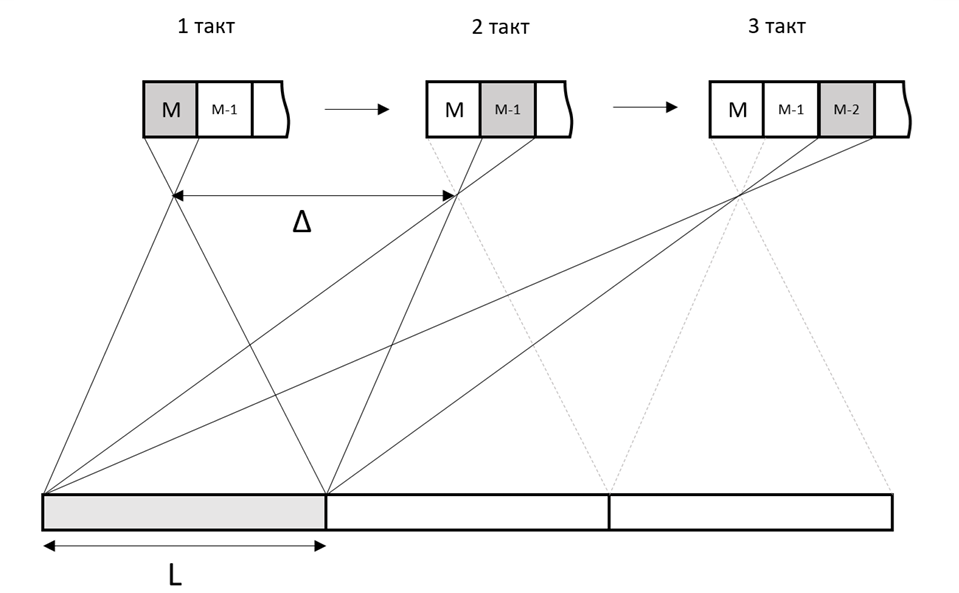
\includegraphics[scale=0.6]{VZN_opt}}
	\caption{Съёмка в режиме ВЗН без \blur{я} ($\tau_T = \tauopt{T}$) }
	\label{fig:VZN_opt}
\end{figure}


В случае, когда программно заданный тактовый период опроса $\tau_T$ оказывается больше оптимального значения $\tauopt{T}$, смещение за время одного такта становится меньше требуемого ($\Delta (\tau_T) < L $). В результате участок сцены проецируется одновременно на два соседних элемента ПЗС-матрицы, и в каждый такт накопления регистрируется сигнал не только от соответствующего участка сцены, но и от смежных областей изображения (Рисунок~\cref{fig:tauT_more}).

\begin{figure}[!h]
	\centerfloat{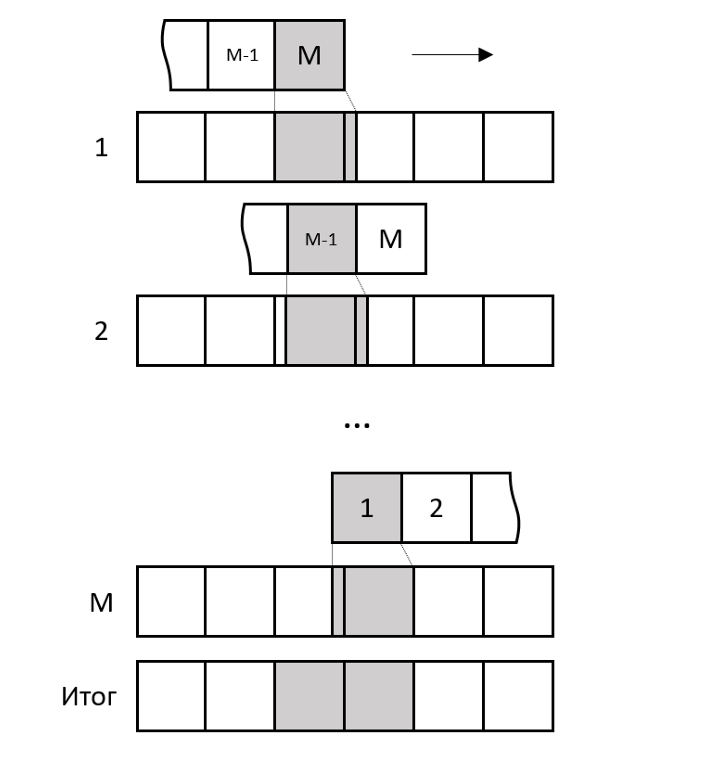
\includegraphics[scale=0.6]{tauT_more}}
	\caption{Возникновение \blur{я} при увеличенном тактовом периоде ($\tau_T > \tauopt{T}$) }
	\label{fig:tauT_more}
\end{figure}

Суммарная территория, участвующая в накоплении сигналов на каждом шаге, оказывается на $\frac{\delta}{M}\cdot L$ больше, чем при съёмке с оптимальным периодом опроса, где $\delta$ -- величина \blur{я} в элементах ПЗС-матрицы, $M$ -- число интеграционных шагов. Таким образом при $\tau_T > \tauopt{T}$ выражение~\eqref{eq:tau_noblur} примет вид:

\begin{equation}
	\label{eq:tau_more_blur}
		\Delta(\tau_T) = L \cdot \frac{(M+\delta)}{M}.
	\end{equation}

Аналогичная ситуация возникает в противоположном случае, когда заданный тактовый период меньше оптимального $\tau_T < \tauopt{T}$. В этом случае смещение изображения за один такт превышает допустимое $\Delta (\tau_T) > L$, и проекция участка сцены смещается быстрее, чем выполняется перенос зарядов. В каждый такт накопления регистрируется лишь часть сигнала от соответствующего участка, а оставшаяся информация теряется между проекциями (Рисунок~\cref{fig:tauT_less}).

\begin{figure}[!h]
	\centerfloat{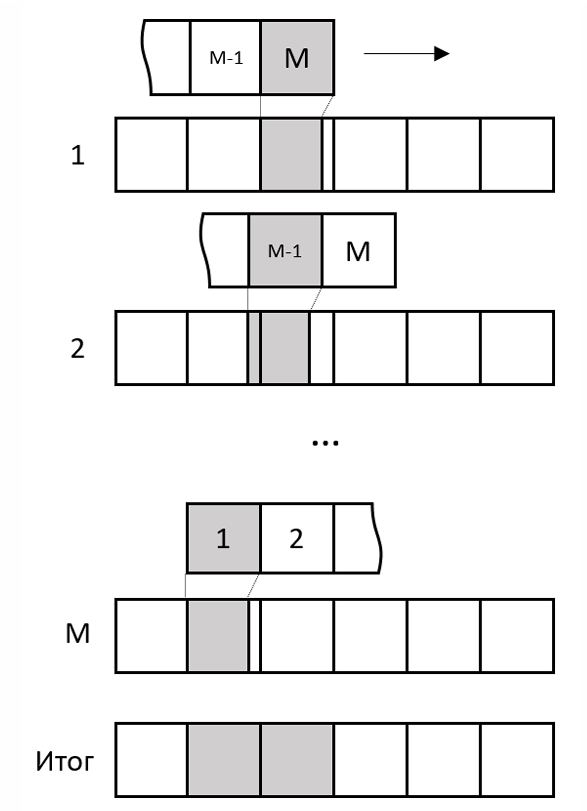
\includegraphics[scale=0.6]{tauT_less}}
	\caption{Возникновение \blur{я} при уменьшенном тактовом периоде ($\tau_T > \tauopt{T}$) }
	\label{fig:tauT_less}
\end{figure}

В результате изображение приобретает фрагментированный характер, снижается резкость и контрастность мелких деталей, выражение~\eqref{eq:tau_noblur} примет вид:
\begin{equation}
	\label{eq:tau_less_blur}
	\Delta(\tau_T) = L \cdot \frac{(M-\delta)}{M}.
\end{equation}

Оптимальный тактовый период опроса определяется по расчётной скорости движения изображения $v_0$:
\begin{equation}
	\label{eq:eq_optimalPeriod}
	\tau_T^* = \frac{L}{v_0} = \frac{l_x m_c}{v_0}.
\end{equation}


Практика эксплуатации показывает, что рассогласование между фактическим и расчётным тактовым периодом может быть вызвано целым комплексом факторов: методическими ошибками при расчёте скорости движения изображения, неточностью поддержания орбитальной и угловой ориентации, температурными деформациями конструкции и вибрациями. Наибольшее влияние в контексте данного исследования оказывают возмущения, возникающие при повороте подвижных частей оптической системы. Вращение оптической системы осуществляется моментом, формируемым приводом, который через механические связи передаёт на корпус космического аппарата реактивный момент. Под его действием изменяется угловая скорость КА, что ведёт к изменению скорости движения изображения на фокальной плоскости:

\begin{equation}
	\label{eq:eq_spdImgae}
	v=f\cdot \omega_{||},
\end{equation}

\noindent  где \(f\) "--- фокусное расстояние оптической системы, \(\omega_{||}\) "--- проекция угловой скорости на направление сканирования.

Изменение скорости изображения приводит к нарушению условия оптимального тактового периода $\tauopt{T}$, в результате чего проекция сцены смещается относительно матрицы приёмника и появляется \blur{е}. В терминах контрастно-частотной характеристики через множители $\text{КЧХ}_{LF}$ и $\text{КЧХ}_{HF}$ в выражении ~\eqref{eq:mtf_total}, которые отражают вклад низко- и высокочастотных колебаний.

Низкочастотные колебания являются наиболее критичным видом динамических возмущений, так как их амплитуда может достигать десятков микрометров, величины сравнимой с размером пикселя~\cite{Wahballah2018}.
В условиях, когда время экспозиции $\exposition$ существенно меньше периода колебаний $T_0$, \blur{е} формируется только на части синусоиды и приобретает квазилинейный характер. При этом величина \blur{я} становится случайной: она зависит от того, на какой фазе колебаний выполняется экспозиция. Минимальное размытие возникает, если экспозиция приходится на экстремум синусоиды, а максимальное  -- когда экспозиция совпадает с точкой нулевого перехода ~\cite{Haghshenas2015a} (рисунок ~\cref{fig:MTF_LF_phase}).

\begin{figure}[!h]
	\centerfloat{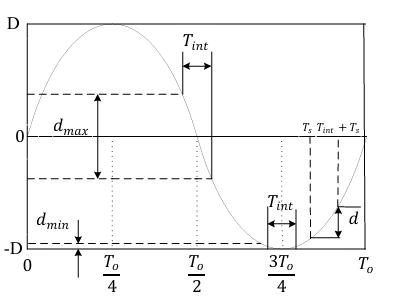
\includegraphics[scale=1]{mtf_lf}}
	\caption{Зависимость величины \blur{а} от фазы низкочастотных колебаний}
	\label{fig:MTF_LF_phase}
\end{figure}

Минимальный и максимальный радиусы \blur{я} определяются выражениями \eqref{blur_min}, \eqref{blur_max}

\begin{equation}
	\label{blur_min}
	d_{min} = D \left( 1 - \cos \left( \frac{2\pi}{T_0} \cdot \frac{T_{int}}{2} \right) \right),
\end{equation} 

\begin{equation}
	\label{blur_max}
	d_{max} = 2D \sin \left( \frac{2\pi}{T_0} \cdot \frac{T_{int}}{2} \right),
\end{equation}

\noindent  где \(D\) "--- амплитуда скорости колебаний, \(\exposition\) "--- время экспозиции, \(T_0\) "--- период колебаний.

Когда траектория смещения изображения в пределах кадра близка к линейной, снижение КЧХ описывается аппроксимацией линейного \blur{я}:

\begin{equation}
	\label{mtf_lf}
	\text{КЧХ}_{LF}(\nu)=\frac{\sin{\pi \nu L}}{\pi \nu L},
\end{equation}

\noindent  где \(L\) "--- величина смещения изображения за время экспозиции, \(\nu\) "--- пространственная частота.

Установлено, что низкочастотные колебания определяют предельное качество изображения. Например при увеличении амплитуды смещения с $1~\text{до}~20~\text{мкм}$ значение КЧХ на частоте Найквиста уменьшается на 41~\%, а при $30~\text{мкм}$ практически падает до нуля~\cite{wahballah2018smear}.

Высокочастотные колебания конструкции космического аппарата обычно возникают из-за дисбалансов реакционных маховиков, дефектов подшипников, работы приводов и упругих резонансов панелей. Характерный диапазон частот для таких возмущений составляет сотни герц и выше, а амплитуда смещений проекции изображения в фокальной плоскости, как правило, не превышает долей микрона (0,2–0,6~мкм) \cite{Haghshenas2015a}. Время экспозиции камеры существенно больше периода колебаний $\exposition \gg T_0$, поэтому результирующее смещение усредняется. 

Для гармонических высокочастотных колебаний КЧХ описывается через функцию Бесселя нулевого порядка:

\begin{equation}
	\label{eq:mtf_hf}
	\text{КЧХ}_{HF}(\nu)=J_0(2\pi \nu D).
	\end{equation}

При малых амплитудах ($D \ll p$, где \(p\)--размер пикселя) КЧХ $\approx 1$


В реальных условиях на движение изображения накладываются несколько высокочастотных гармоник. При суперпозиции двух синусоидальных гармоник итоговое значение КЧХ снижается сильнее, хотя деградация остаётся существенно меньше по сравнению с низкочастотными возмущениями.


В случае случайных высокочастотных колебаний, связанных с микродрожанием конструкции и шумами приводов, используется гауссова аппроксимация \cite{Holst2008}:

\begin{equation}
	\label{eq:mtf_rand}
	\text{КЧХ}_{HF}(\nu) = \exp\!\left(-2 \pi^2 \sigma_R^2 \nu^2 \right),
	\end{equation}

\noindent где \(\sigma_R\) "--- среднеквадратичное дрожание изображения.


Таким образом, высокочастотные вибрации вносят менее выраженный, но всё же значимый вклад в деградацию изображения. Их влияние становится критическим при совпадении спектра колебаний с резонансами конструктивных элементов КА или при наложении нескольких гармоник. Однако в большинстве практических сценариев $\text{КЧХ}_{HF}$ остаётся близкой к единице, а решающим ограничивающим фактором качества выступают низкочастотные колебания, описываемые через $\text{КЧХ}_{LF}$.

Характер воздействия реактивного момента на качество изображения можно условно разделить на три составляющих. Первая — низкочастотная, связанная с медленным изменением угловой скорости при выполнении манёвра. Она изменяет среднее значение скорости движения изображения, смещая систему из оптимального режима съёмки. Вторая — гармоническая, возникающая из-за колебаний элементов конструкции или резонансов в системе ориентации, которые могут поддерживаться вращающимися деталями исполнительных механизмов. Третья — случайная, обусловленная нерегулярными импульсами момента при работе приводов и механическими шумами. Все три компоненты вносят вклад в снижение функции передачи модуляции и интегральных показателей качества.

\section{Методы компенсации реактивного момента}
Возмущающий момент, возникающий при работе приводов подвижных частей космических аппаратов, является одним из ключевых факторов, ограничивающих точность наведения и стабилизации. Для снижения его влияния применяются различные методы компенсации, которые условно можно разделить на механические и алгоритмические. В основе большинства решений лежит идея создания дополнительного вращающегося или инерционного элемента, формирующего момент, противоположный возмущающему.

В мировой практике для компенсации реактивных моментов применяются различные технические и алгоритмические решения: использование реакционных маховиков и гиродинов \cite{pittelkau2012pointing, dennehy2021spacecraft}, балансировка подвижных узлов \cite{alvarez2018spacecraft}, а также специальные законы управления приводами, формирующие сглаженные профили разгона и торможения \cite{lappas2002attitude, zhao2023effect}. Дополнительно рассматриваются методы цифровой коррекции смаза на изображениях — геометрические, спектральные и градиентные, среди которых наиболее перспективными для реализации на борту являются градиентные подходы \cite{volobuev2021dissertation}. Эти меры позволяют снизить спектр возмущений в критически значимых диапазонах частот, однако минимизация их влияния на формируемое изображение остаётся актуальной задачей исследований.

Наиболее простым и широко используемым способом является применение компенсирующего маховика, вращающегося во встречном направлении относительно основного привода. При этом создаётся противодействующий момент, позволяющий снизить суммарное воздействие на основание конструкции. Правильный подбор инерционных характеристик маховика обеспечивает уменьшение низкочастотной составляющей возмущений, возникающих при разгоне и торможении нагрузки, а также частичную компенсацию гармонических возмущений. Подобная схема используется в системах наведения оптических приборов и антенн, где требуется высокая точность удержания линии визирования \cite{montenbruck2002satellite}. Ограничением метода является необходимость размещения дополнительного узла и обеспечения его синхронной работы с основным приводом, что увеличивает массу, энергопотребление и сложность управления.

Другим конструктивным решением является использование двухприводных систем. В этом случае нагрузка перемещается с помощью двух двигателей, установленных симметрично относительно центра масс. Каждый двигатель создаёт собственный реактивный момент, но благодаря зеркальному расположению и синхронизации вращения они взаимно компенсируются. Такой подход снижает передачу возмущений на корпус аппарата и уменьшает требования к жёсткости несущей конструкции. Применение двухприводных схем было предложено в ряде исследовательских проектов для систем наведения антенн и высокоточных зеркальных механизмов \cite{worthington2010design}. Недостатком является усложнение системы управления, необходимость точного согласования работы приводов и усложнение конструкции.

Одним из оригинальных инженерных решений, направленных на исключение передачи возмущающего момента на корпус космического аппарата, являются приводы с подвижным статором. В таких конструкциях статор двигателя не жёстко закреплён, а установлен на подшипниках и может свободно поворачиваться вокруг оси ротора. Реактивный момент, возникающий при работе ротора, приводит к вращению статора, который через редуктор или напрямую соединён с маховиком-компенсатором. Последний создаёт уравновешивающий момент, противоположный по направлению к моменту от ротора. Таким образом достигается полное исключение передачи реактивного момента на основание. Питание обмоток статора осуществляется через скользящие токоподводы, что усложняет конструкцию, но позволяет реализовать компактный узел с высокой степенью компенсации возмущений~\cite{RU2646002C2}. Другим направлением развития являются двигательные приводы с редукторами, применяемые, в частности, для наведения антенн и солнечных батарей. В патенте~\cite{RU2466069C2} описана конструкция электропривода с редуктором, обеспечивающая высокую долговечность и точность позиционирования за счёт применения гармонического или планетарного редуктора в сочетании с преднатянутыми подшипниками. Такая схема позволяет минимизировать люфты и компенсировать тепловые деформации в условиях длительной работы в космосе. Основным эффектом является значительное снижение передачи вибраций и случайных колебаний на корпус аппарата при сохранении высокого крутящего момента на выходе редуктора.

Важным направлением во всех описанных приводах является использование балансировочных устройств, которые позволяют уменьшить динамические возмущения за счёт устранения эксцентриситета и неидеальной балансировки роторов. Для этого на подвижные элементы устанавливаются специальные балансировочные грузы или кольца, компенсирующие смещение центра масс. Такой подход позволяет эффективно снизить как гармонические, так и случайные составляющие возмущающего момента. Особенно актуальны эти меры в системах с быстро вращающимися деталями, где даже незначительный дисбаланс приводит к формированию высокочастотных вибраций, передающихся на корпус и ухудшающих характеристики оптико-электронной аппаратуры. В ряде работ продемонстрировано, что правильно подобранные балансировочные элементы способны существенно уменьшить уровень микровибраций \cite{liu2008reaction,alcorn2018fully}. Ограничением метода является то, что он в основном устраняет статические и динамические дисбалансы, но не способен компенсировать момент, возникающий непосредственно от управляющих воздействий на привод.

Помимо конструктивных решений, активно развиваются алгоритмические методы компенсации. Их суть заключается в формировании такого закона управления приводом, при котором динамические возмущения минимальны. Наиболее известными являются S-образные, синусоидальные и другие сглаженные профили ускорения, которые ограничивают спектр возбуждаемых гармоник и предотвращают возникновение резонансов в конструкции. Алгоритмическая компенсация особенно эффективна для снижения случайной составляющей реактивного момента, обусловленной нерегулярными импульсами момента при работе привода и механическими шумами. В публикации \cite{singer1990preshaping,singhose2009command} показано, что правильно выбранный профиль управления позволяет существенно снизить остаточные возмущения без введения дополнительных механических элементов, что делает метод перспективным для лёгких и маломощных космических аппаратов. Однако его эффективность зависит от точности модели системы и качества обратной связи, поэтому в реальных условиях полного устранения возмущений добиться не удаётся.

Таким образом, существующие методы компенсации реактивного момента охватывают широкий спектр решений: от введения дополнительных механических узлов до оптимизации управляющих воздействий. Каждое из них имеет свои преимущества и ограничения. Наиболее эффективной на практике является комбинация механических и алгоритмических средств, обеспечивающая одновременное снижение как низкочастотной и гармонической составляющих, так и случайных возмущений. Однако вследствие технологических и конструктивных ограничений полностью устранить воздействие не удаётся, и в системе всегда остаётся остаточный реактивный момент, который подлежит регистрации и последующей оценке.


\subsection{Компенсация реактивного момента}

Для компенсации реактивного момента, возникающего при разгоне и торможении инерционных объектов (зеркал, оптических сборок и др.), может применяться активная электромеханическая схема с соосным компенсирующим приводом. Принципиальная идея заключается в установке второго ротора с динамикой, противоположной по направлению основной нагрузке. При равенстве динамических моментов обоих приводов результирующее воздействие на корпус спутника обращается в ноль:

\begin{equation}
	\label{eq:equal_inertia}
	J_1\frac{d\omega_1}{dt}+J_2\frac{d\omega_2}{dt} = 0,
\end{equation}


\noindent где \(J_1,J_2\)"--- моменты инерции подвижных частей, \(\omega_1,\omega_2\)"--- угловые скорости.

На практике конфигурация может быть реализована как с двумя независимыми двигателями, так и с использованием редукторной связи между основным и компенсирующим ротором. Применение редуктора позволяет снизить массу маховика, так как эквивалентный момент инерции уменьшается пропорционально квадрату коэффициента передачи $i$.

Особое внимание при проектировании систем компенсации реактивного момента уделяется трению в шарикоподшипниках, которое в условиях космоса становится главным источником сопротивления. Даже при отсутствии атмосферы и силы тяжести момент трения сохраняется за счёт предварительного натяга, центробежных и гироскопических сил. Проблема точной оценки момента трения особенно важна при разработке приводов оптико-механических систем, где остаточный реактивный момент напрямую влияет на качество изображения. В ряде работ~\cite{Babaeva1962, Delektorskii1968, Shashanov1971,Yavlensky1981} отмечено, что суммарный момент $M_{\text{тр}}$ в подшипниках включает две основные составляющие: момент трения от нагрузки $M_0$ и гидродинамическую составляющую смазки $M_1$. При этом именно $M_1$ во многих случаях оказывается доминирующим~\cite{Mikhailov2014}. Для количественной оценки момента трения в радиально-упорных шарикоподшипниках изделий космического назначения используются уточнённые эмпирические зависимости. Согласно работе~\cite{Delektorskii1968}, суммарный момент трения может быть представлен следующим образом:

\begin{equation}
	\label{eq:Mtr}
	M_{\text{тр}} = M_0 + M_1 = 0{,}6 \cdot 10^{-3} A_0
	\frac{D_0}{d_{\text{ш}}} \cdot \frac{1}{\sqrt[3]{z d_{\text{ш}}}}+4{,}41 \cdot 10^{-6} \cdot D_0^3 n,
\end{equation}
где \(A_0\)"--- осевой преднатяг, \(D_0\)"--- средний диаметр подшипника, \(d_{\text{ш}}\)"--- диаметр шарика, \(z\)"--- число шариков, \(n\)"--- скорость вращения.
	
Формула (\ref{eq:Mtr}) даёт удовлетворительное совпадение с экспериментальными данными (погрешность не превышает 20 \%), что позволяет использовать её для инженерных расчётов при проектировании приводов и маховиков в космических аппаратах.

Характерным является наличие момента трогания $M_{\text{трог}}$, который превышает установившийся момент сопротивления в среднем в $1,5-2$ раза~\cite{Mikhailov2014}. Это приводит к скачкообразной передаче момента на корпус спутника в момент пуска. При несовпадении значений $M_{\text{трог}}$ у основного и компенсирующего приводов возникает остаточное возмущение, вызывающее угловой дрейф. Для снижения влияния момента трогания применяются конструктивные и технологические меры. Наиболее распространённым методом является предварительная обкатка подшипников, позволяющая снизить $M_{\text{трог}}$ в 2–3 раза и повысить стабильность его значения во времени~\cite{Mikhailov2014}. Существенное влияние оказывает выбор смазки: использование консистентных смазок с оптимальной вязкостью позволяет уменьшить разброс значений момента трогания между подшипниками. Важным является и обеспечение высокой точности обработки дорожек качения, что снижает локальные пики сопротивления при запуске.Со стороны систем управления эффект момента трогания компенсируется формированием специальных профилей разгона с контролируемым нарастанием момента. Это позволяет синхронизировать работу основного и компенсирующего приводов и уменьшить риск возникновения остаточного момента.

Однако, даже при использовании соосных компенсирующих приводов и учёте особенностей трения в подшипниках полностью устранить остаточный реактивный момент не удаётся. Его величина определяется как конструктивными факторами (точность изготовления, свойства смазки, качество сборки), так и алгоритмами управления приводами. Поэтому для корректной оценки влияния возмущающих моментов на динамику космического аппарата необходимо не только их моделирование, но и прямые экспериментальные измерения.

\section{Измерение реактивного момента}


С точки зрения механики сплошных сред, крутящий момент можно определить как произведение силы на плечо её приложения:

\begin{equation}
	\label{eq:eq_Torque}
	M=F \cdot r,
\end{equation}
где \(F\) "--- приложенная сила, \(r\) "--- расстояние от точки приложения силы до оси вращения.

Для вала круглого сечения при кручении момент связан с углом закручивания $\phi$ выражением:

\begin{equation}
	\label{eq:eq_torque}
	M=G\cdot J \cdot \frac{\phi}{L},
\end{equation}
где \(G\) "--- модуль сдвига материала, \(J\) "--- полярный момент инерции сечения, \(L\) --- длина участка.

Именно эта зависимость лежит в основе многих методов измерения момента -- фиксируется угол закручивания или напряжённое состояние материала, а затем по известным параметрами конструкции вычисляется величина момента.

Современные датчики крутящего момента реализуются на основе более чем десяти различных физических принципов. Наиболее распространённые из них:
\begin{itemize}
	\item Тензорные датчики -- основаны на измерении деформации упругого элемента с помощью тензорезисторов. Отличаются высокой точностью, но требуют установки датчика в разрыв вала\cite{yeh2015digital,Hou2009,Mohammed2008,Chen2020}.
	\item магнито-упругие -- используют эффект изменения магнитной проницаемости материала под действием кручения. Недостаток -- чувствительны к внешним полям \cite{Shu2007}.
	\item Оптоволоконные датчики с решётками Брэгга -- фиксируют микродеформации с высоким разрешением, однако требуют намотки волокна на вал и потому не являются полностью бесконтактными \cite{Zhu2021}
	\item Пьезоэлектрические и фотоупругие датчики -- преобразуют механическую деформацию в электрический сигнал, могут быть миниатюрных размеров, но ограничены по диапазону измерения \cite{Bojtos2017,Hu2020}.
	\item Оптические методы -- обеспечивают бесконтактность и высокую точность, но подвержены влиянию вибрации \cite{Garinei2017,Sjodahl1996}
\end{itemize}
Несмотря на разнообразие подходов, все методы делятся на две большие категории:
\begin{itemize}
	\item Контактные датчики -- взаимодействуют с объектом напрямую, интегрируются в конструкцию. Они обеспечивают высокое качество измерений, но изменяют характеристики самой системы.
	\item Бесконтактные датчики -- не оказывают механического воздействия, удобны для встроенного мониторинга, но ограничены по разрешению и устойчивости к возмущениям \cite{Wang2021}. 	
\end{itemize} 

Контактные методы применимы для широкого диапазона задач, но в высокоточных системах (робототехника, аэрокосмические приводы, микро-механизмы) критично минимизировать их влияние на конструкцию. Бесконтактные оптические методы обладают рядом преимуществ: высокой точностью, нечувствительностью к температурным и электромагнитным помехам, малым влиянием на исследуемую систему. Однако они традиционно сталкиваются с проблемой устойчивости к радиальным вибрациям и ограничениями по диапазону.

В качестве примера современных тенденций в этой области можно привести исследование \cite{Chen2024}, где предложен новый бесконтактный метод измерения момента, основанный на оптической когерентной интерферометрии. Принцип заключается в нанесении микрошкал на поверхность вала (ширина порядка 62,8 мкм), которые служат физической картой деформаций. Оптическая система регистрирует смещения шкал при закручивании вала, а специальные алгоритмы обработки сигнала (быстрое преобразование Фурье и метод энергетического центра Ханнинга) обеспечивают разрешение вплоть до 0,003 Н·м. Несмотря на то, что данный метод не используется в рамках настоящей работы, он иллюстрирует направление развития современных бесконтактных технологий измерения момента.

Большинство существующих методов ориентировано на измерение момента непосредственно в точке приложения привода, то есть на его валу. В отличие от локального крутящего момента, который характеризует работу конкретного исполнительного узла и фиксируется в месте передачи энергии, реактивный момент проявляется как отклик на основании или несущей конструкции и отражает интегральное воздействие привода на систему в целом. В космических приложениях ключевым становится именно измерение реактивного момента, так как он определяет динамические возмущения, передающиеся на корпус аппарата и влияющие на точность ориентации в пространстве.

Для снижения возмущений реактивный момент обычно компенсируется с помощью дополнительного маховика, вращающегося в противоположном направлении. Однако компенсация никогда не является полной: вследствие несовершенства балансировки и нелинейностей в системе остаётся остаточный реактивный момент. Его регистрация и количественная оценка необходимы для анализа устойчивости системы и корректного прогнозирования влияния привода на работу всего аппарата.

В доступной литературе практически отсутствуют исследования, посвящённые детальному расчёту и, в особенности, непосредственному измерению реактивного момента, возникающего при вращении подвижных частей оптико-электронной аппаратуры космического назначения. В немногочисленных публикациях, где рассматривается вопрос измерений, регистрация реактивного момента, как правило, осуществляется на валу привода или двигателя \cite{Rayanov2020}, что отражает лишь локальное крутильное воздействие в месте установки датчика. Однако такой подход не позволяет получить эквивалентный полный вектор реактивного момента, передаваемого на корпус космического аппарата, поскольку не учитываются дополнительные компоненты, возникающие вследствие смещений центра масс, инерционного взаимодействия подвижного узла с несущими элементами конструкции, а также динамических эффектов в механизмах передачи движения. Наиболее близким по постановке задачи к настоящему исследованию является метод определения возмущающего момента, реализованный на инерционном стенде для экспериментальной отработки системы наведения антенн космического аппарата \cite{Goncharuk2013}. Рассмотрим этот метод подробнее. Конструкция стенда представлена на рисунке ~\cref{fig:stand}.
\begin{figure}[ht] 
	\centerfloat{
		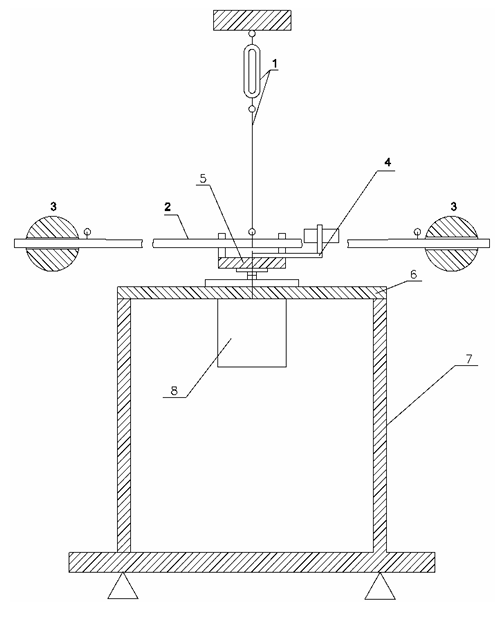
\includegraphics[scale=0.8]{stand} 
	}
	\legend{1 – система обезвешивания; 2 – штанга; 3 – груз; 4 – датчик угловой скорости с кронштейном для установки; 5 – элемент для передачи момента на выходной вал; 6 – плита установочная; 7 – основание; 8 – объект контроля}
	\caption{Функциональная схема инерционного стенда}
	\label{fig:stand} 
\end{figure}

Метод определения возмущающего момента, реализованный в рассмотренной работе, %todo переписать соавторов
основан на использовании инерционного стенда, позволяющего воспроизводить динамические характеристики системы наведения антенн космического аппарата в наземных условиях. Конструктивно стенд представляет собой основание с закреплённой на нём плитой, на которой устанавливается механический привод антенны. К выходному валу привода присоединяется имитатор нагрузки, выполненный в виде штанги с грузами, масса и положение которых подбираются таким образом, чтобы эквивалентный момент инерции соответствовал параметрам реальной антенны. Для снижения влияния силы тяжести используется система обезвешивания, а инерционный имитатор позволяет воспроизводить упругие и динамические свойства навешиваемого оборудования. Регистрация параметров движения осуществляется с помощью датчика угловой скорости, установленного непосредственно на выходном валу привода. В процессе эксперимента фиксируется изменение угловой скорости при различных режимах работы — как при равномерном вращении, так и в переходных процессах разгона и торможения. Полученные зависимости $\omega(t)$ подвергаются дифференцированию для вычисления углового ускорения, после чего возмущающий момент определяется по выражению:
\begin{equation}
	\label{eq:eq_M_disturb}
	M=J_{\text{н}}\cdot \frac{d\omega}{dt},
\end{equation}
где \(J_{\text{н}}\) "--- момент инерции имитируемой нагрузки, \(\omega\) "--- угловая скорость.

Таким образом, метод сводится к регистрации динамики вращения исполнительного механизма и последующему вычислению возмущающего момента через известные параметры имитируемой нагрузки.

Применение данного метода позволяет оценить возмущающее воздействие, создаваемое приводом в установившихся и переходных режимах, а также проанализировать их спектральные характеристики.

Несмотря на несомненные достоинства, описанный метод имеет ряд ограничений, которые не позволяют использовать его в рамках настоящего исследования. Прежде всего следует отметить, что стенд оперирует не реальной нагрузкой, а её имитатором, выполненным в виде штанги с грузами. Для каждой конкретной аппаратуры требуется изготавливать отдельный имитатор с заданным моментом инерции, и даже при тщательной калибровке всегда сохраняется погрешность в воспроизведении динамических характеристик реального узла. Кроме того, сам принцип измерений остаётся локальным: возмущающий момент определяется по данным датчика, установленного на валу привода, тогда как для задач космической техники критическим является именно реактивный момент, передаваемый на корпус КА. Такой подход не позволяет получить полное представление о суммарном воздействии на конструкцию в реальных условиях работы. Наконец, существенным ограничением является невозможность воспроизведения ситуации, когда одновременно вращаются и нагрузка, и компенсирующий маховик. Регистрация реактивного момента после компенсации имеет принципиальное значение для оценки качества динамики в высокоточных оптико-электронных системах. В совокупности, эти факторы делают метод, реализованный на инерциальном стенде, недостаточным для решения поставленной в настоящей работе проблемы.

\section*{Выводы по главе 1}
В первой главе рассмотрено современное состояние исследований в области динамических воздействий на оптико-электронные системы космических аппаратов и их влияние на качество формируемых изображений. Показано, что повышение разрешающей способности и внедрение механизмов поворота визирной оси без разворота аппарата сопровождается ростом требований к стабилизации изображения и одновременно приводит к усилению динамических возмущений, вызванных перемещением подвижных масс.

Анализ показал, что реактивный момент, возникающий в результате работы приводов, является одним из ключевых факторов, снижающих качество изображений. Его влияние проявляется через три компоненты: низкочастотную, гармоническую и случайную. Все они приводят к смещению скорости движения изображения на фокальной плоскости относительно оптимального значения, что вызывает \blur{е} и дрожание изображения, а также снижает интегральные показатели качества, включая КЧХ и Image Quality Factor.

Для снижения воздействия реактивного момента применяются различные методы компенсации, включая компенсирующие маховики, двухприводные механизмы, балансировочные устройства и алгоритмическую компенсацию на уровне законов управления. Эти решения позволяют уменьшить спектр возмущений в критических диапазонах частот, однако полностью устранить их влияние не удаётся. В системе неизбежно остаётся остаточный реактивный момент, который требует учёта и оценки.

Обзор существующих методов измерения крутящего момента показал, что они в основном ориентированы на регистрацию момента на валу двигателя. Такой подход отражает только локальное крутильное воздействие и не эквивалентен реактивному моменту, передаваемому на корпус космического аппарата. Рассмотренный метод экспериментальной отработки на инерционном стенде позволяет оценить возмущающие моменты привода, однако он основан на использовании имитатора нагрузки и не учитывает работу компенсирующих маховиков, а потому не позволяет регистрировать остаточный реактивный момент всей системы.

Таким образом, выполненный анализ подтвердил, что в доступной литературе практически отсутствуют исследования, посвящённые непосредственному измерению реактивного момента подвижных частей оптико-электронной аппаратуры космического назначения. Этот пробел обосновывает необходимость разработки специализированных методов регистрации и анализа остаточного реактивного момента, что и составляет предмет настоящего исследования.

\FloatBarrier

